
%% HUH Colloquium Presentation
%% Tom Eichlersmith

\documentclass{beamer}

\mode<presentation> {
	\usetheme{Goettingen}
	\setbeamertemplate{navigation symbols}{}
	\setbeamertemplate{footline}[page number]
}

\usepackage{graphicx} % Allows including images
\usepackage{booktabs} % Allows the use of \toprule, \midrule and \bottomrule in tables
\usepackage{subfigure} % For images next to each other

%-----------------------------------------------
%%	TITLE PAGE
%-----------------------------------------------

\title[HUH Colloquium]{Honors Colloquium} % The short title appears at the bottom of every slide, the full title is only on the title page

\author{Tom Eichlersmith}
\institute[Hamline U]
{
Hamline University \\
\medskip
\textit{teichlersmith01@hamline.edu}
}
\date{\today}

\begin{document}

\begin{frame}
\titlepage % Print the title page as the first slide
\end{frame}

\begin{frame}
\frametitle{Overview} % Table of contents slide, comment this block out to remove it
\tableofcontents % Throughout your presentation, if you choose to use \section{} and \subsection{} commands, these will automatically be printed on this slide as an overview of your presentation
\end{frame}

%------------------------------------------------
%%	PRESENTATION SLIDES
%------------------------------------------------

\section{HUH Overview} 

\subsection{Academic Excellence} % A subsection can be created just before a set of slides with a common theme to further break down your presentation into chunks

\begin{frame}
	
\frametitle{Academic Excellence}

\begin{figure}[h]
	
\includegraphics[width=0.8\linewidth]{images/clock.png}
\end{figure}

\end{frame}

%------------------------------------------------

\subsection{Research Experience}

\begin{frame}
\frametitle{Research Experience}

\begin{itemize}
	\item Piezoelectric Energy Harvesting
	\item Search for Harmonic Drums
	\item Forward Proton Simulations
	\item Random Walks on Simple Surfaces
\end{itemize}

\begin{figure}
	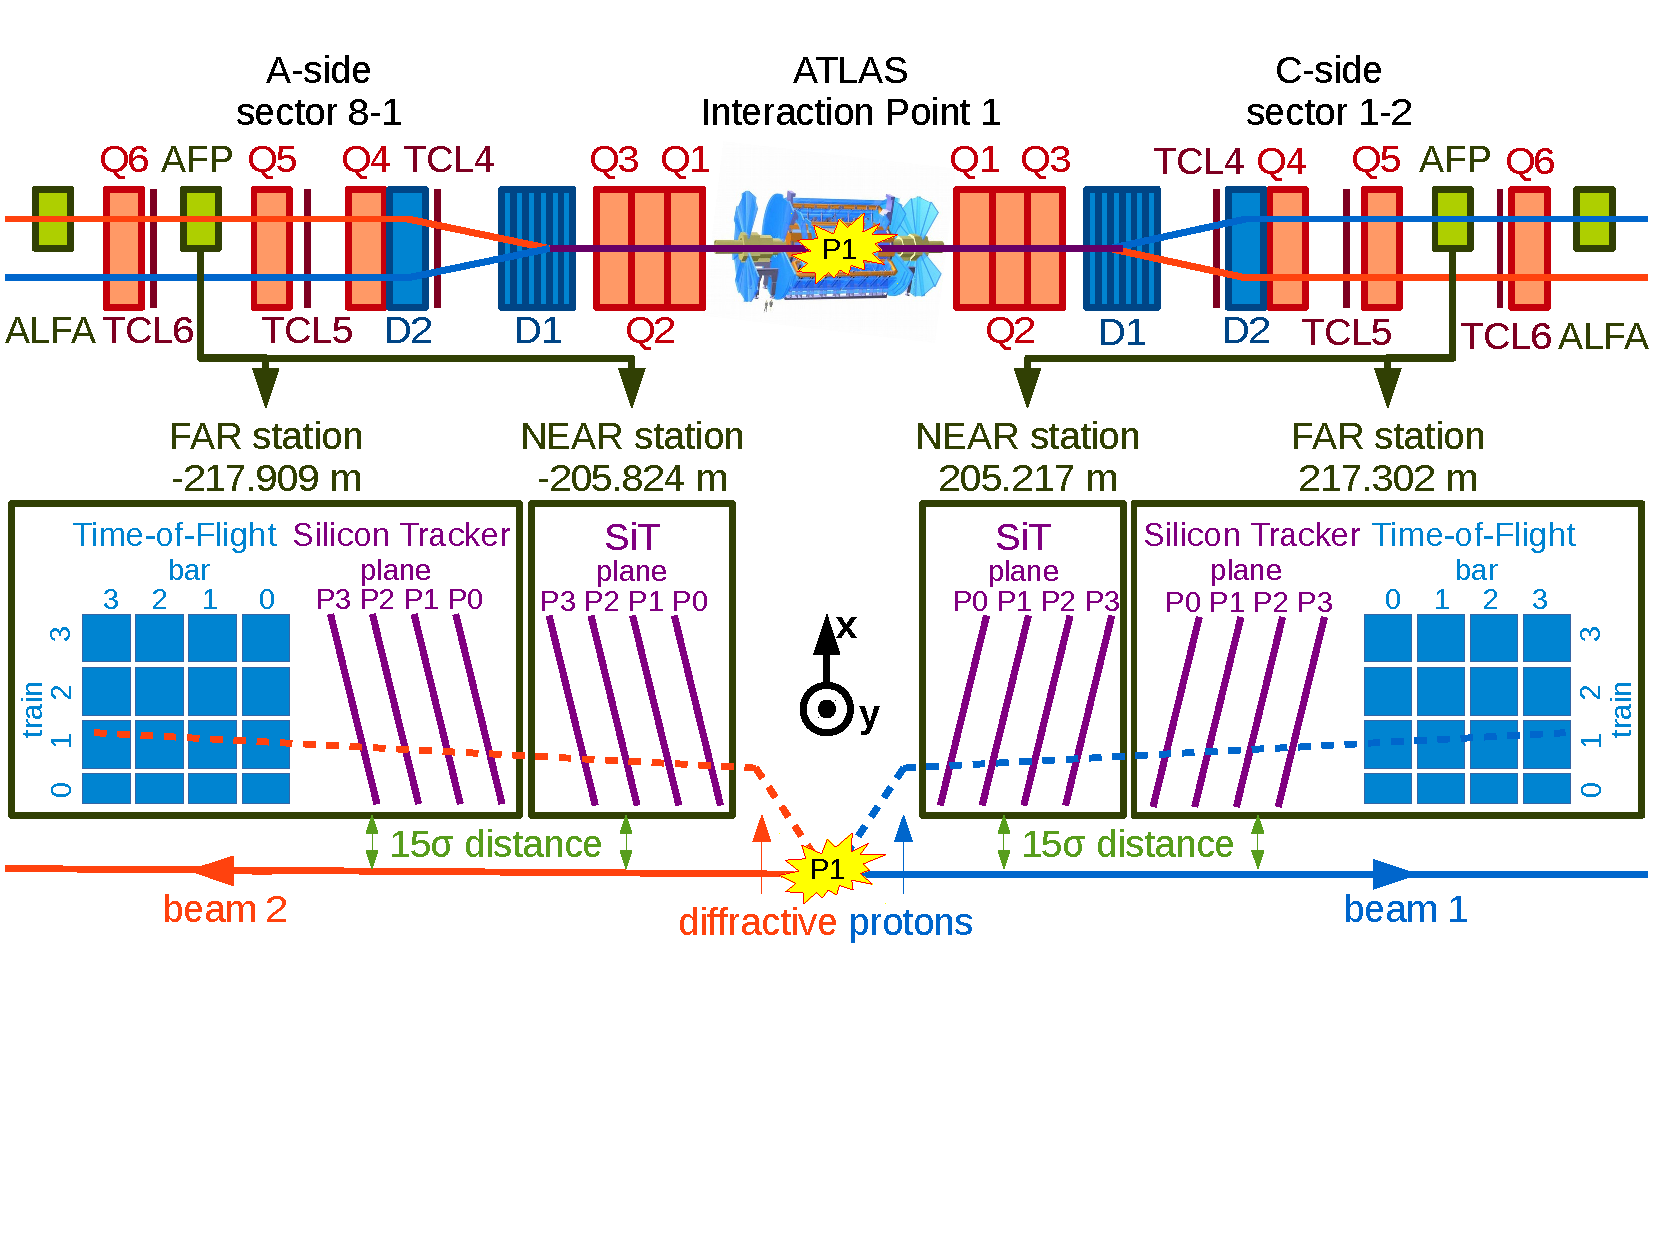
\includegraphics[width=0.7\linewidth]{images/afp_general_scheme.pdf}
	\caption{M. Trzebinski \texttt{twiki.cern.ch/twiki/bin/view/Atlas/AFP\_Figures} }
\end{figure}

\end{frame}

%------------------------------------------------

\subsection{Contributions to Community}

\begin{frame}
\frametitle{Contributions to Community}

\begin{itemize}
	\item Radio Station
	%MUSIC IMAGE
	\item Programming Board
	%HUPB GRAPHICS
\end{itemize}

\end{frame}

%------------------------------------------------

\subsection{Development as a Lifelong Learner}

\begin{frame}
\frametitle{Development as a Lifelong Learner}

\end{frame}

%------------------------------------------------
\section{Specific Experience}
%------------------------------------------------

\begin{frame}
\frametitle{Planning Winter Wonder Jam}
\begin{figure}[htp]
	\centering
	\subfigure{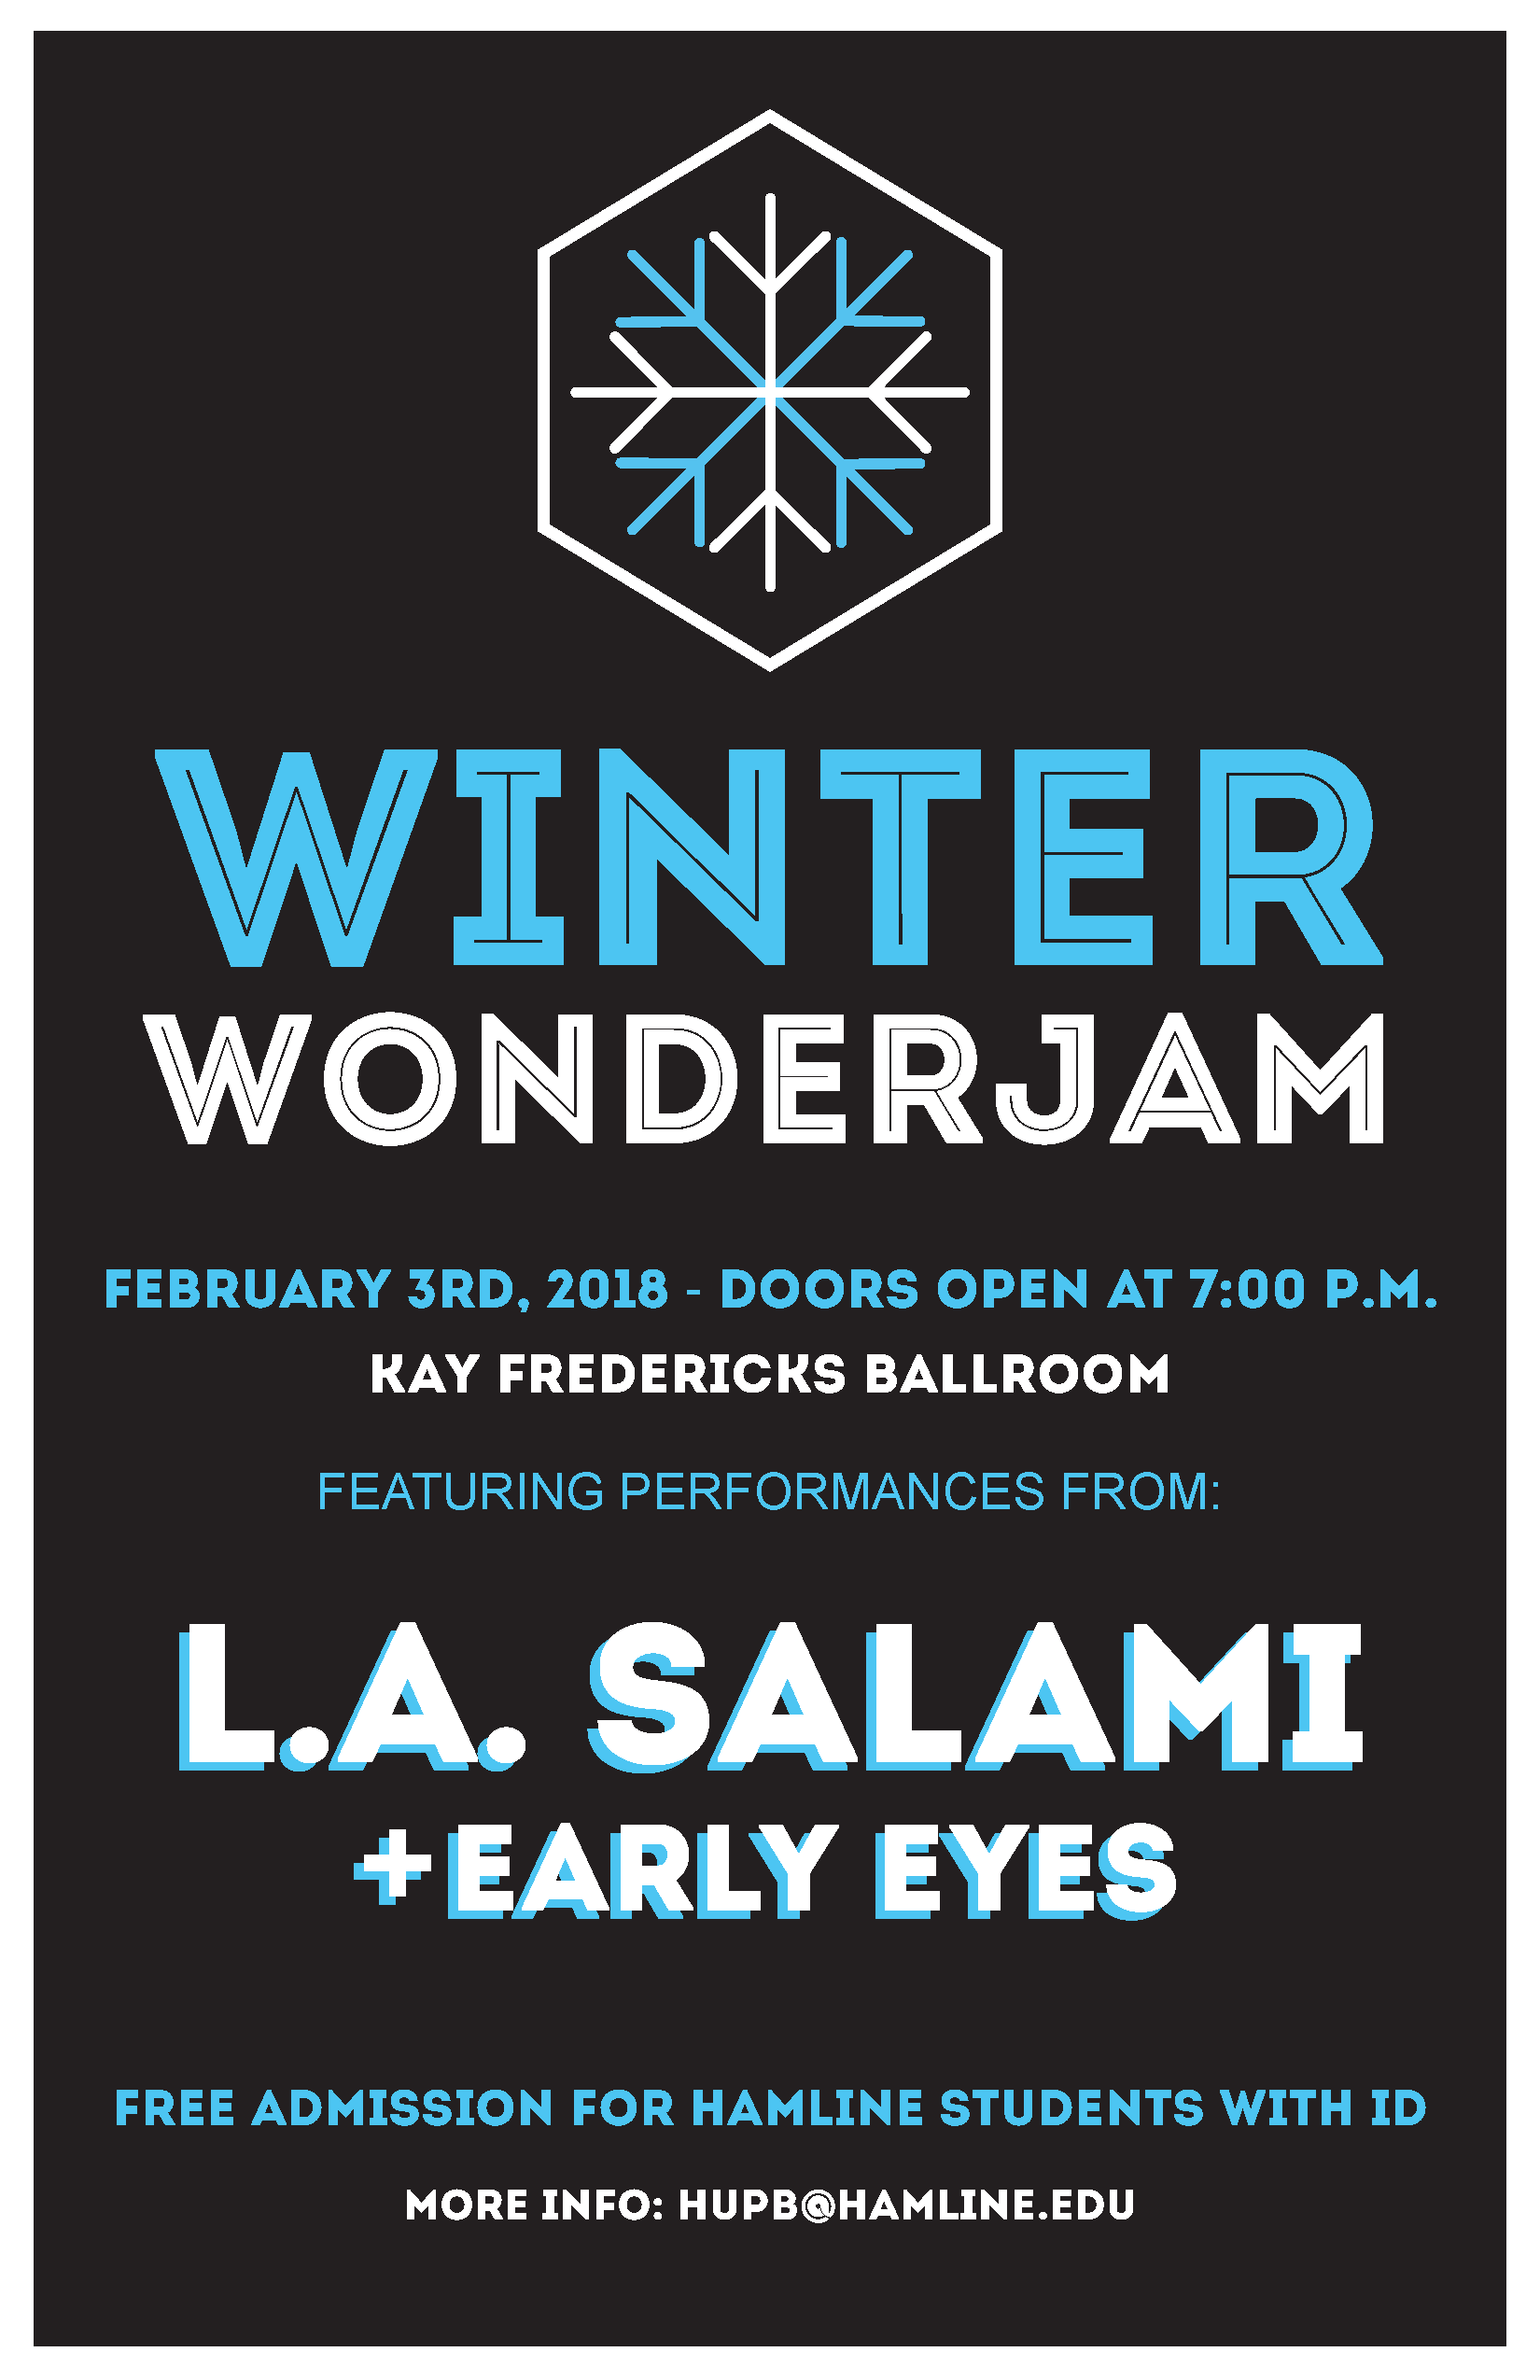
\includegraphics[width=0.4\textwidth]{images/WWJ_18.pdf}}
	\quad
	\subfigure{
\includegraphics[width=0.4\textwidth]{images/WWJ_17.png}}
\end{figure}
\end{frame}

%------------------------------------------------

\section{Connection of Different Pillars}

\begin{frame}
\frametitle{Connection of Different Pillars}

\end{frame}

%------------------------------------------------

\section{HUH Impact and My Future}

\begin{frame}
\frametitle{HUH Impact and My Future}

\end{frame}

%------------------------------------------------

\section{Questions}

\begin{frame}
\Huge{\centerline{Questions?}}
\end{frame}

%------------------------------------------------

\end{document} 